\chapter{Lec 17 - Machine Learning I}
\section{What is Machine Learning}
\textit{A computer program is said to learn from experience E with respect to some class of tasks T and performance measure P, if its performance at tasks in T, as measured by P, improves with experience E.} Basically, Machine Learning is the field of study that gives computers the ability to learn without being explicitly programmed. In fact, we use Machine Learning when its impossible to \textbf{exactly formalise} the problem (and so to give an algorithmic solution) or when formulating a solution it's very complex and cannot be done manually.\\\\
There are three ingredients for a learning algorithm:
\begin{itemize}
    \item The Task
    \item The Performance Measure
    \item The Experience
\end{itemize}
A \textbf{task} is usually described in terms of how the machine learning algorithm should process an example. There are several different tasks:
\begin{itemize}
    \item Classification
    \item Regression
    \item Machine translation
    \item ...
\end{itemize}
The \textbf{performance measure} depends on the task and measures how good is our model trained using the learning algorithm. For example: for a classification task, a good performance measure can be the \textbf{accuracy}, i.e.,  the proportion of examples for which the model produces the correct output. For a regression task, the performance measure can be the \textbf{mean squared error} (MSE), i.e.,  the average of the squares of the errors.\\\\
The \textbf{experience} is the set of data on which we train our model. These data can be real-valued, discrete or mixed and they can be obtained once for all (batch learning), or acquired incrementally by interacting with the environment (on-line learning).\\\\
There are several ways in which data can be used to learn.

\subsection{Main Learning Paradigms}
\begin{itemize}
    \item \textbf{Supervised Learning:}
    \begin{itemize}
        \item \textbf{Goal: }give the \textit{right answer} for each example in the data.
        \item Given a training set $\{(x^{(i)}, y^{(i)})\}$ we look for a function $h(\cdot)$ which is able to map in a predictive way $x^{(i)}$'s to $y^{(i)}$'s. It's called supervised learning because there is an expert that provides a \textit{supervision} assigning a label $y^{(i)}$ to each input $x^{(i)}$ 
        \item \textbf{Output: }Classification, regression.
        \item Use cases: Object recognition, Predicting pandemic, ... 
    \end{itemize}
    \begin{center}
        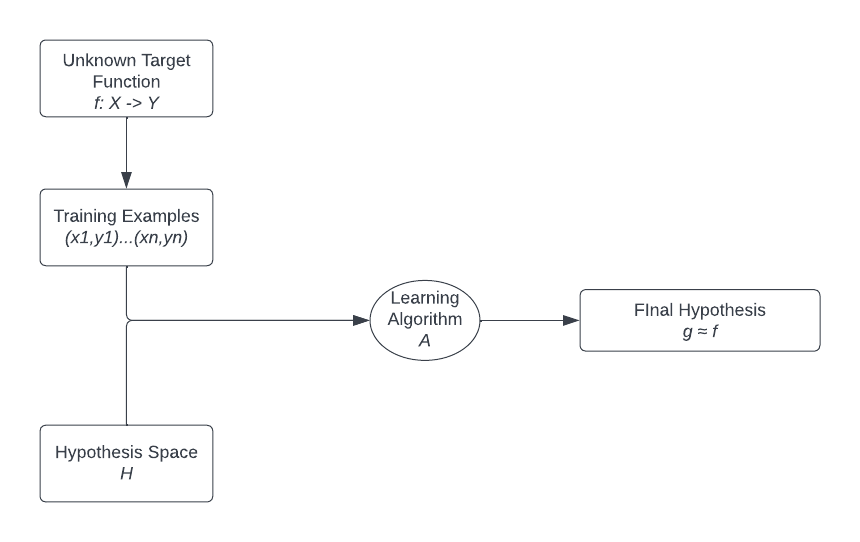
\includegraphics[scale=0.8]{images/Supervised Learning Diagram.png}
    \end{center}
    The \textit{Training examples} are generated according to the \textit{Target function $f$} (unknown). Once we have this set of pairs, we choose the \textit{hypothesis space}. The \textit{learning algorithm} (e.g a Neural Network) searches in the hypothesis space for a function $g$ that approximates the target function $f$.
    \item \textbf{Unsupervised Learning:}
    \begin{itemize}
        \item \textbf{Goal:} Find regularities / patterns on the data
        \item Given examples $\{x^{(i)}\}$, discover regularities on the whole input domain.
        \item There is no supervision.
        \item Use cases: Community detection in social media, user profiling, market analysis ...
    \end{itemize}    
    \item \textbf{Reinforcement Learning:}
    An \textbf{Agent} operates in an environment $e$, which in response to action $a$ (given by the agent) in the state $s$ returns the next state and a reward $r$ (which can be positive, negative or neutral).
    The goal of the Agent is to maximize a reward function.
    \begin{itemize}
        \item Use cases: Robotics, Games, ...
    \end{itemize}
    \begin{center}
        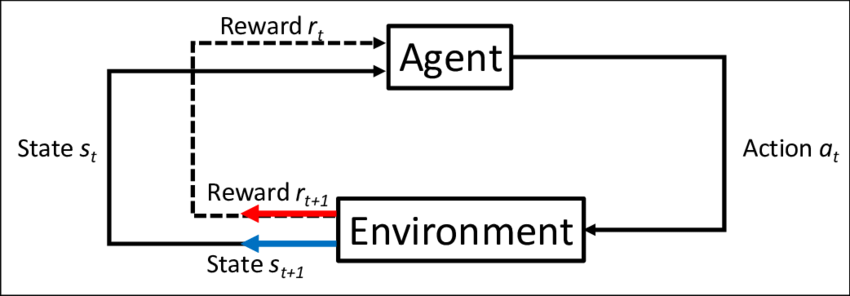
\includegraphics{images/Reinforcement learning.png}
    \end{center}
    \item \textbf{Other Learning Strategies:}
    \begin{itemize}
        \item Active Learning
        \item Online Learning, Incremental \& Continual Learning
        \item Weak Supervised Learning
        \item Self-supervised Learning
        \item Deep Learning and Representation Learning
        \item Federated Learning
    \end{itemize}
\end{itemize}

\section{Fundamental Ingredients}

\begin{itemize}
\item \textbf{Input/Instance space x $\in X$:}
Representation of model's input (e.g. you can choose a Vector as a representation for your input). It contains all the possible inputs for a model. Suppose the model takes in a vector, $input = [x1, x2], x1,x2 \in [1,10]$, then we have $10^2$ possible inputs.
\item \textbf{Output space $y \in Y$:}
In supervised learning we want to perform a prediction based on the input. This prediction can be in the form of:
\begin{itemize}
    \item Binary Classification $y \equiv \{-1, +1\}$
    \item Multi-Class Classification $y \equiv \{1,...,m\}$
    \item Regression $y \equiv \mathbb{R}$
\end{itemize}
\item \textbf{Oracle/Nature:}
It determines how examples are generated. We can have two cases of Oracle
\begin{itemize}
    \item Target function $f: X \rightarrow Y$ It's deterministic and given an object of the input space returns an object of the output space. This function is ideal and \textbf{unknown}.
    \item Probability distribution $P(\textbf{x}), P(y\mid\textbf{x})$ The \textit{selection} of $y$ occurs from a probability distribution. This distribution is still unknown
\end{itemize}
\item \textbf{Training set:}
Set of pairs $\{(\textbf{x}_{1}, y_{1}), ..., (\textbf{x}_{n}, y_{n}) \}$ where each pair is composed by an instance of the input space and it's corresponding label.
\begin{center}
    \begin{tabular}{c|c}
     \textbf{x} & y\\
     000&0  \\
     001&1 \\
     010&1 \\
     .&. \\
     .&. \\
     .&.\\
    \end{tabular}
\end{center}

\item \textbf{Hypothesis space:}
A \textbf{predefined} set of hypothesis/functions $H \equiv \{h\mid h:X \rightarrow Y\}$. It constitutes the set of functions which can be implemented by the machine learning system. It is assumed that the function to be learned $f$ may be
approximated by a hypothesis $h \in H$. Note that $H$ cannot coincide with the set of all possible functions and the search (into $H$) to be exhaustive, otherwise there would be infinitely many functions that fit the training data and $h$ would just memorize the training data.\\\\
For this reason we must make assumptions about the type of the unknown target function. The \textbf{inductive bias} consists of:
\begin{itemize}
    \item The hypothesis space: how $H$ is defined
    \item The learning algorithm: how $H$ is explored
\end{itemize}
Let's see some examples of hypothesis space.
\begin{itemize}
    \item \textbf{Hyperplanes in} $\mathbb{R}^{2}$: We chose as input space points in the plane $X = \{y\mid y \in \mathbb{R}^{2}\}$, and as hypothesis space the dichotomies induced by hyperplanes in $\mathbb{R}^{2}$, that is, $H = \{f_{w,b}(y) = sign(\textbf{w} \cdot y + b), \textbf{w} \in \mathbb{R}^{2}, b \in\mathbb{R}\}$.
    \begin{center}
        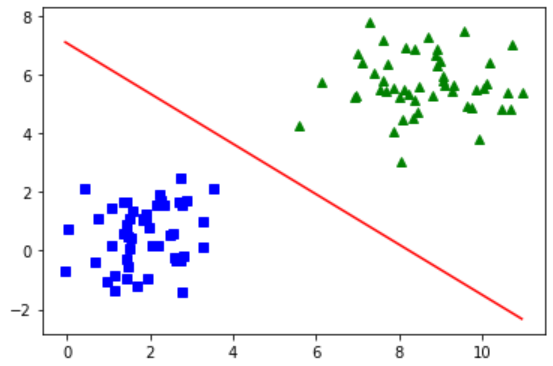
\includegraphics{Hyperplanes in R^2}
    \end{center}

    
    \item \textbf{Polynomial functions}:
    Given a training set $S = \{(x_{1},y_{1}),...,(x_{n}, y_{n})\}, x\in \mathbb{R}, y\in \mathbb{R}$, the hypothesis space is the one containing functions of type: $h_{w}(x) = w_{0} + w_{1}x + w_{2}x^{2} + ... + w_{p}x^{p}, p\in \mathbb{N}$.
    \begin{center}
        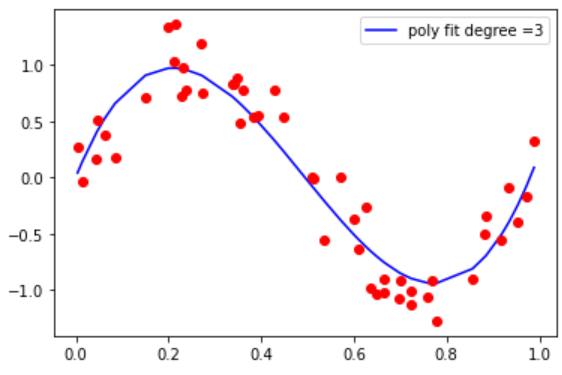
\includegraphics{images/Poly reg.png}
    \end{center}
\end{itemize}
\end{itemize}

\section{Example of Learning Algorithm: Perceptron}
Consider the space of hyperplanes in $\mathbb{R}^{n}$, where $n$ is the dimension of the input.
\[H = \{f_{(\textbf{w},b)}(\textbf{x}) = sign(\textbf{w} \cdot \textbf{x} + b): \textbf{w,x} \in \mathbb{R}^{n}, b \in \mathbb{R}\}\]
where $\textbf{w}$ is a vector of weights and $b$ is the \textbf{bias} term.\newline\newline
We can redefine $H$ as:
\[H = \{f_{\textbf{w}^{'}}(\textbf{x}^{'}) = sign(\textbf{w}^{'} \cdot \textbf{x}^{'}): \textbf{w}^{'}, \textbf{x}^{'} \in \mathbb{R}^{n+1}\}\]
after the following change of variables:
\[\textbf{w}^{'} = [b, \textbf{w}], \quad \textbf{x}^{'} = [1, \textbf{x}]\]
it follows that:
\[\textbf{w}^{'} \cdot \textbf{x}^{'} = b + \sum_{i = 1}^{n}\textbf{w}_{i}\textbf{x}_{i} = \textbf{w} \cdot \textbf{x} + b\]
Basically, we add a dimension to $\textbf{w}$ and $\textbf{x}$ just to simplify the notation of $H$.
\begin{center}
    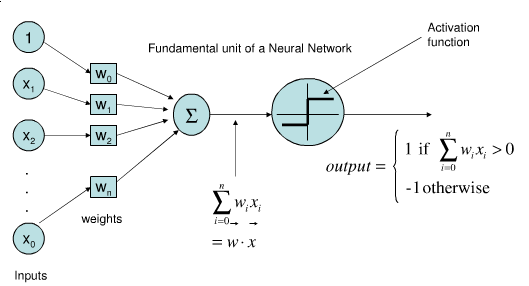
\includegraphics[scale=0.5]{images/perceptron.png}
\end{center}
The model described in the image above is called \textbf{Perceptron}. It first computes the dot-product between the weights $\textbf{w}$ and the input $\textbf{x}$. The result of this computation is usually called $net$
\[net = \sum_{i=0}^{n}w_{i}x_{i}\]
The final output is obtained by applying the \textbf{step function} to the $net$.
\[o = \sigma(net) = sign(net)\]
We will refer to this neuron (and associated learning algorithm) as Perceptron.\newline\newline
Since the hypothesis space of the Perceptron is defined as the hyperplanes in $\mathbb{R}^{n}$, it converges only if the examples in $\mathbb{R}^{n}$ are \textbf{linearly separable}. Otherwise, it will never \textit{find} a hyperplane that separates them.
\subsection{Perceptron: learning algorithm}
Assume to have training examples in $\mathbb{R}^{n}$ that are linearly separable:\newline\newline
Input: Training set $S = \{(\textbf{x}, t), \textbf{x} \in \mathbb{R}^{n+1}, t \in \{-1, +1\}, \eta \geq 0\}$
\begin{enumerate}
    \item Initialize the value of the weights $\textbf{w}$ randomly;
    \item Repeat (N epochs)
    \begin{enumerate}
        \item Select (randomly) one of the training examples $(\textbf{x}, t)$
        \item if $o = sign(\textbf{w} \cdot \textbf{x}) \neq t$ then
        \[\textbf{w} \leftarrow \textbf{w} + \eta(t-o)\textbf{x}\]
    \end{enumerate}
\end{enumerate}
A small value of the learning rate $\eta$ can make the learning process slow but more stable, that is, it prevents sharp changes in the weights vector. If the training set is linearly separable, it can be shown that the Perceptron training algorithm terminates in a finite number of steps.\\\\
Let’s try to define a linear model that predicts the XOR function:
\[Tr = \{ ([0,0], 0), ([0, 1], 1), ([1,0],1), ([1,1], 0)\]
The XOR function \textbf{cannot} be learned by any linear classifier. In order to solve this problem, we would need a more complex hypothesis space (e.g. Neural network).
\begin{center}
    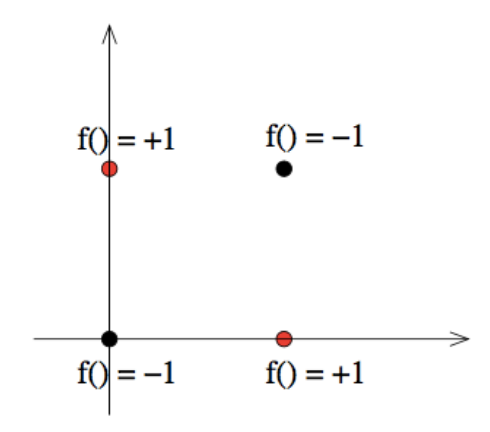
\includegraphics[scale=0.8]{images/xor.png}
\end{center}

\section{Empirical/True Error}
The \textbf{Empirical Error} $error_{Tr}(h)$ of hypothesis $h$ with respect to $Tr$ is the number of examples that $h$ misclassifies.\\\\
The \textbf{True Error} $error_D(h)$ of hypothesis $h$ with respect to target concept $c$ and distribution $D$ is the probability that $h$ will misclassify an instance drawn according to $D$. This can only be estimated. One way to estimate this quantity is testing the model over new examples that are not in the training set (test set).
\[error_D(h) \equiv Pr_{x \in D}(c(x) \neq h(x))\]
$h \in H$ \textbf{overfits} $Tr$ if $\exists h' \in H$ such that $error_{Tr}(h) < error_{Tr}(h')$, but $error_D(h) > error_D(h')$.

\section{Hypothesis Space Complexity}
Let's consider a plane with 4 points. If we choose the hyperplanes in $\mathbb{R}^{2}$ as hypothesis space $H$ we can divide the points with a line and classify them with two colors (red and green). These partitions are called dichotomies. Note that this particular $H$ \textbf{can't} implement all possible dichotomies.
\begin{center}
    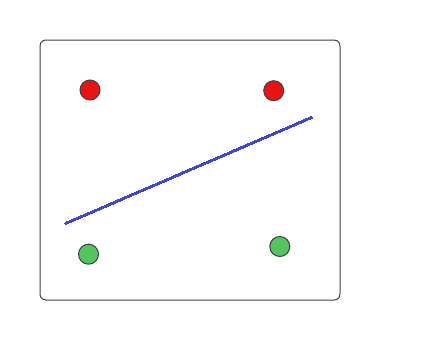
\includegraphics{images/Dichotomy 1.png}
    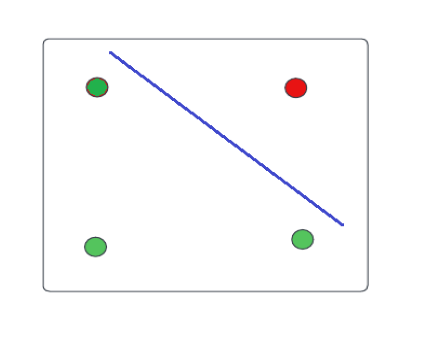
\includegraphics{images/Dichotomy 2.png}
\end{center}

\begin{figure}[h]
    \centering
    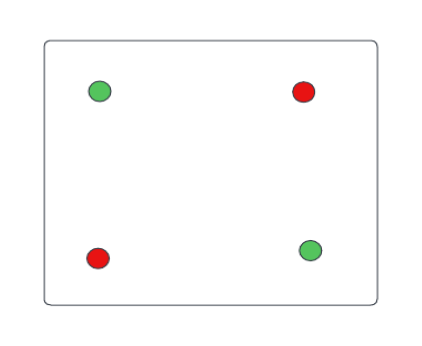
\includegraphics{images/Dichotomy 3.png}
    \caption{This classification can't be implemented by any hyperplane in $H$}
\end{figure}

\begin{itemize}
    \item \textbf{Shattering: } Given $S \subset X, S$ is shattered by the hypothesis space $H$ iff 
    \[\forall S^{'} \subseteq S, \exists h \in H, s.t. \forall x \in S, h(x) = 1 \iff x \in S^{'}\]
    That means that $H$ is able to implement all possible dichotomies of $S$.
    
    \item \textbf{VC-dimension: } The VC-dimension of an hypothesis space $H$ defined over an instance space $X$ is the size of the largest finite subset of $X$ shattered by $H$: 
    \[VC(H) = \max_{S \subseteq X}|S|\]
    such that S is shattered by $H$.
\end{itemize}
If we consider $H_{1} = \{f_{w,b}(y) | f_{w,b}(y) = sign(w \cdot y + b), w \in \mathbb{R}^{2}, b \in \mathbb{R}\}$ as hypothesis space (hyperplanes in $\mathbb{R}^{2}$), $VC(H_{1}) = 3$ because it doesn't exist \textbf{any} configuration of 4 points that can be shattered by $H_{1}$. If we consider just three points, there are $2^3 = 8$ possible dichotomies, and there exists \textbf{at least} one configuration which is shattered by $H_1$.
\begin{center}
    \includegraphics[scale=0.6]{images/dichotomy 3.png}
\end{center}
In general, VC-dimension of hyperplanes in $\mathbb{R}^{n} = n + 1$: in 2 dimensions $VC(H) = 3$, in 3 dimensions $VC(H) = 4$ and so on.
